\chapter{Metodi}
Questo capitolo tratterà le tecnologie, gli strumenti, le librerie e gli algoritmi utilizzati per la realizzazione dei modelli predittivi e dell’interfaccia successivamente creata. 
\section{Tecnologie utilizzate}
\subsection{Machine Learning}

Il Machine Learning, o apprendimento automatico, è un campo di studio che si occupa di sviluppare algoritmi in grado di perfezionarsi automaticamente mediante l'esperienza acquisita tramite l'utilizzo dei dati. 

Gli algoritmi di Machine Learning creano modelli matematici a partire da dati di esempio chiamati "dati di training", in modo da poter attuare predizioni o prendere decisioni senza essere esplicitamente programmati per farlo. 

Esistono tre categorie di approcci di Machine Learning: l'apprendimento supervisionato, l'apprendimento non supervisionato e l'apprendimento per rinforzo.
\begin{itemize}
    \item L'apprendimento supervisionato consiste nell’indicare al calcolatore una regola generale che mappi gli input e gli output desiderati. 
    
    L'algoritmo di apprendimento è provvisto di dati di input di esempio e degli output corrispondenti e, attraverso successive iterazioni, viene successivamente costruito un modello matematico che può essere sfruttato per predire l'output associato ad un nuovo input.
    
    \item L'apprendimento non supervisionato invece, non fornisce all'algoritmo di apprendimento le etichette desiderate. 
    
    In questo caso, l'algoritmo di apprendimento deve necessariamente estrapolare le informazioni significative dai dati di input pur non essendo a conoscenza dell'output desiderato.
    
    \item L'apprendimento per rinforzo prevede che un programma interagisca con un ambiente dinamico con lo scopo di raggiungere un obiettivo specifico, ad esempio guidare un veicolo o vincere un gioco contro un avversario. 
\end{itemize}
Durante le varie iterazioni il programma riceve un feedback sotto forma di premio e cerca di massimizzare il suo “punteggio”, in modo da imparare e raggiungere l'obiettivo prefissato.

\subsection{Computer Vision}
La Computer Vision è un campo interdisciplinare che si occupa della capacità dei computer di acquisire conoscenza da immagini o video, cercando di replicare il complesso meccanismo alla base dell'apparato visivo umano. 

Questa utilizza metodi per l'acquisizione e l'analisi di immagini digitali in modo da estrarre dati multidimensionali dal mondo reale e produrre informazioni numeriche o simboliche. 

Si avvale pertanto anche di conoscenze di geometria, fisica, statistica e della teoria dell'apprendimento per descrivere il mondo in modo sensato, producendo risultati che possono indirizzarci alla corretta linea d'azione.

\subsection{Cuda}
[da https://developer.nvidia.com/cuda-zone]
CUDA® è una piattaforma di calcolo parallelo, un modello di programmazione sviluppato da NVIDIA per il calcolo generale su unità di elaborazione grafica (GPU). 

Per mezzo di CUDA, gli sviluppatori possono ampliare significativamente la velocità delle applicazioni di calcolo sfruttando la potenza delle GPU.

Nelle applicazioni dotate di accelerazione GPU, la parte sequenziale del carico di lavoro viene eseguita sulla CPU, ottimizzata per le prestazioni single-threaded, mentre la parte computazionalmente intensiva dell’applicazione viene realizzata su migliaia di core GPU in parallelo. 

Quando ci si avvale di CUDA, gli sviluppatori hanno la possibilità di programmare in linguaggi popolari come C, C++, Fortran, Python e MATLAB, esprimendo il parallelismo attraverso estensioni sotto forma di poche parole chiave di base.
Il toolkit CUDA di NVIDIA fornisce tutto il necessario per sviluppare applicazioni con accelerazione GPU.

Il toolkit CUDA include librerie accelerate su GPU, un compilatore, strumenti di sviluppo e il runtime CUDA.

\begin{figure}
    \begin{center}    
        
\includegraphics[width=0.9\linewidth]{images/image1.png}
    \end{center}
\end{figure}

\section{Strumenti utilizzati}
\subsection{Visual Studio Code}
Visual Studio Code è un editor di testo sviluppato da Microsoft per Windows, Linux e macOS, che supporta il debugging, il controllo Git integrato, la Syntax Highlighting, l'IntelliSense, lo Snippet e il refactoring del codice. 

Visual Studio Code supporta molteplici linguaggi e funzionalità aggiuntive grazie alla possibilità di installare dei plugin disponibili attraverso un repository centrale che presenta, oltre a diverse estensioni fornite direttamente da Microsoft, innumerevoli estensioni rese disponibili dalla community. 

\begin{figure}[h]
    \begin{center}
        \begin{minipage}[b]{0.35\linewidth}
            \centering
            
\includegraphics[width=\linewidth]{images/image2.png}
        \end{minipage}
        \begin{minipage}[b]{0.35\linewidth}
            \centering
            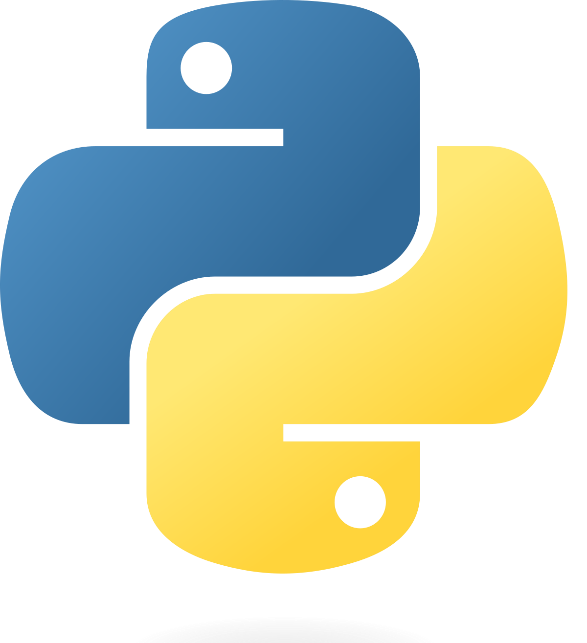
\includegraphics[width=\linewidth]{images/image3.png}
        \end{minipage}
    \end{center}
\end{figure}

\section{Librerie utilizzate}
\subsection{Pandas}
La libreria software open source Pandas è stata sviluppata per il linguaggio di programmazione Python, ed è utilizzata per la manipolazione e l'analisi dei dati. Con Pandas è possibile effettuare operazioni su tabelle numeriche e serie temporali mediante le sue strutture dati. 

Il termine"Pandas" deriva dal termine econometrico "Panel Data", appellativo attribuito a un insieme di dati contenenti osservazioni sugli stessi individui durante più periodi di tempo.

\begin{figure}
    \begin{center}    
        
\includegraphics[width=0.9\linewidth]{images/image4.jpeg}
    \end{center}
\end{figure}

\subsection{Tqdm}
[da https://tqdm.github.io/]
La libreria Python tqdm è uno strumento molto utile per la visualizzazione di barre di avanzamento durante i cicli di elaborazione nel codice. 

Il nome "tqdm" deriva dall'unione della parola araba "taqaddum" che significa "progresso" ed è l'abbreviazione di "te quiero demasiado" (ti amo troppo) in spagnolo. 

Per servirsi della libreria basta inserire qualsiasi iterabile (liste, dizionari, tuple e set) nel metodo della libreria, in questo modo \mintinline[bgcolor=bg]{python}{tqdm(iterable)}. 

La libreria funziona su qualsiasi piattaforma ed è completamente indipendente dalle dipendenze. 

Durante l'estrazione delle Action Units la libreria tqdm ha fornito una stima precisa del tempo necessario per completare l'elaborazione, consentendo di monitorare l'avanzamento del processo in tempo reale. 

Nonostante l'utilizzo della tecnologia CUDA per accelerare le analisi, la grande quantità di immagini da elaborare ha richiesto molto tempo. 

La presenza di tqdm è stata quindi di fondamentale importanza, in quanto ha permesso di gestire efficacemente l'elaborazione dei dati, evitando eventuali problemi tecnici, garantendo risultati accurati ed affidabili e portandomi a riconsiderare delle scelte algoritmiche, non efficientissime, prese. 

In sintesi, la libreria Python tqdm è uno strumento prezioso per semplificare l'elaborazione di grandi quantità di dati, fornendo una stima del tempo rimanente e consentendo di pianificare il lavoro in modo efficiente.

\begin{figure}
    \begin{center}    
        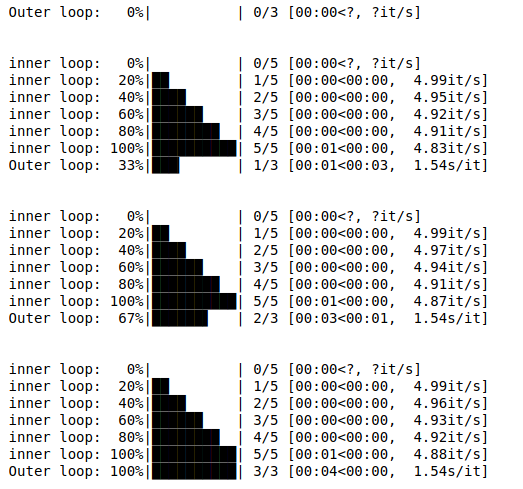
\includegraphics[width=0.9\linewidth]{images/image5.png}
    \end{center}
\end{figure}

\subsection{Pickle}
La libreria pickle è molto versatile e può essere utilizzata per salvare e ripristinare qualsiasi tipo di oggetto Python, inclusi dizionari, liste, tuple, classi e istanze di oggetti personalizzati. 

Inoltre, pickle supporta anche la serializzazione di oggetti multipli in un unico file, rendendo più semplice l'organizzazione dei dati. 

La libreria offre anche diverse opzioni per controllare il comportamento della serializzazione, come la scelta del protocollo di serializzazione e la possibilità di escludere alcuni attributi dall'oggetto da serializzare.

Una caratteristica importante della libreria pickle è che gli oggetti serializzati possono essere utilizzati su diverse piattaforme e versioni di Python, purché il protocollo di serializzazione utilizzato sia compatibile. 

Ciò significa che un oggetto serializzato su un computer Windows con Python 3.9 può essere deserializzato su un computer Linux con Python 2.7, ad esempio. 

Tuttavia, è importante notare che non tutti gli oggetti possono essere serializzati correttamente, come ad esempio le funzioni e le istanze di oggetti di alcune librerie Python. 

Inoltre, la compatibilità tra diverse versioni di Python non è garantita in tutti i casi; quindi, è necessario prestare attenzione a eventuali incompatibilità.

\begin{figure}
    \begin{center}    
        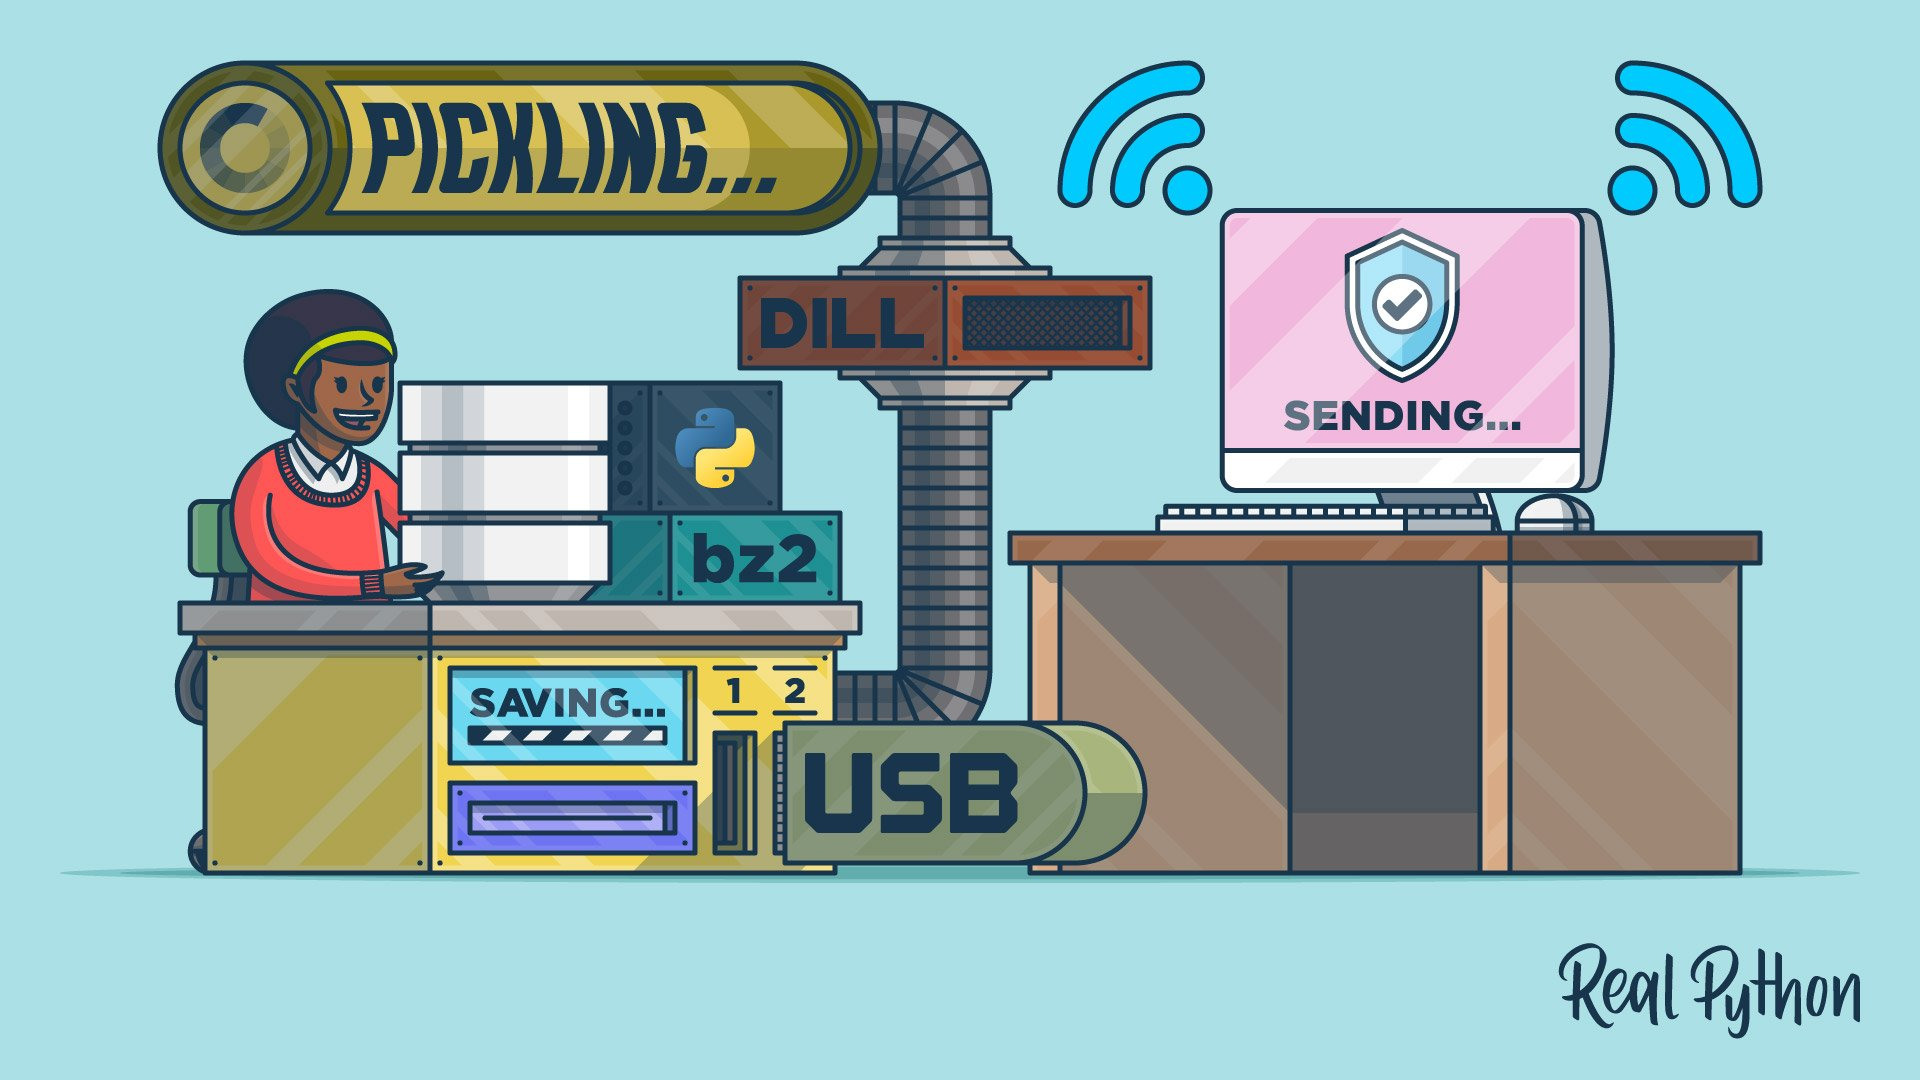
\includegraphics[width=1\linewidth]{images/image6.jpeg}
    \end{center}
\end{figure}

\subsection{Torch}
PyTorch è un popolare framework open-source di deep learning che consente agli sviluppatori di creare modelli di intelligenza artificiale in modo rapido ed efficiente. È stato sviluppato originariamente da Facebook AI Research, guadagnandosi una grande popolarità per la sua facilità d'utilizzo, la sua flessibilità e la sua scalabilità.

Una delle sue principali caratteristiche è la sua architettura a flusso di dati (data flow), la quale rende il framework particolarmente adatto per le applicazioni di deep learning. 

Inoltre, PyTorch è dotato di un'ampia gamma di librerie e strumenti come PyTorch Lightning, che mirano a semplificare lo sviluppo di modelli di intelligenza artificiale.

Questa libreria è anche conosciuta per la sua flessibilità e scalabilità, in quanto permette di creare modelli di deep learning sia per computer singoli che per cluster di computer. 

In aggiunta, supporta una vasta gamma di piattaforme hardware, come CPU, GPU e TPU, il che la rende adatta per le applicazioni in ambiti come il machine learning, la visione artificiale e il linguaggio naturale.

\begin{figure}
    \begin{center}    
        
\includegraphics[width=0.9\linewidth]{images/image7.png}
    \end{center}
\end{figure}

\subsection{OpenCV}
[Da https://opencv.org/about/]
OpenCV (Open Source Computer Vision Library) è una libreria software open source finalizzata all’ambito della computer vision e del machine learning. 

È stata ideata per fornire un'infrastruttura comune per le applicazioni di computer vision e per accelerare l'uso della percezione automatica nei prodotti commerciali. 

In quanto prodotto con licenza Apache 2, OpenCV facilita l'utilizzo e la modifica del codice da parte delle aziende.

La libreria contiene più di 2500 algoritmi ottimizzati, che includono un insieme completo di algoritmi di computer vision e machine learning sia classici che all'avanguardia. 

Questi algoritmi possono essere utilizzati per:
\begin{itemize}
  \item rilevare e riconoscere volti, 
  \item identificare oggetti, 
  \item classificare azioni umane nei video, 
  \item tracciare il movimento della telecamera, 
  \item tracciare oggetti in movimento, 
  \item estrarre modelli 3D di oggetti, 
  \item produrre cluster di punti 3D da telecamere stereo, 
  \item unire immagini per produrre un'immagine ad alta risoluzione di un'intera scena, 
  \item trovare immagini simili da un database di immagini, 
  \item rimuovere gli occhi rossi dalle immagini scattate con il flash, 
  \item seguire i movimenti degli occhi, 
  \item riconoscere paesaggi,
  \item creare marker per sovrapporli alla realtà aumentata, ecc. 
\end{itemize}

OpenCV ha più di 47mila utenti nella sua comunità e un numero stimato di download superiore a 18 milioni.

Oltre alle aziende ben consolidate come Google, Yahoo, Microsoft, Intel, IBM, Sony, Honda e Toyota, esistono molte startup come Applied Minds, VideoSurf e Zeitera che ne fanno un uso intensivo. 

Esso è impiegato per molteplici applicazioni, tra cui unire immagini di Street View, rilevare intrusioni in video di sorveglianza in Israele, monitorare l'equipaggiamento minerario in Cina, aiutare i robot a navigare e raccogliere oggetti presso Willow Garage, rilevare gli incidenti di annegamento in piscina in Europa, eseguire arte interattiva in Spagna e New York, controllare le piste di atterraggio per rilevare detriti in Turchia, ispezionare le etichette sui prodotti nelle fabbriche di tutto il mondo e per la rapida rilevazione dei volti in Giappone.

È provvisto di interfacce per C++, Python, Java e MATLAB e supporta Windows, Linux, Android e Mac OS. 

Attualmente sono in sviluppo interfacce complete per CUDA e OpenCL. 

Ci sono oltre 500 algoritmi e circa 10 volte tante funzioni che compongono o supportano questi ultimi.

OpenCV è scritto nativamente in C++ e ha un'interfaccia template che funziona perfettamente con i contenitori STL.

\begin{figure}
    \begin{center}    
        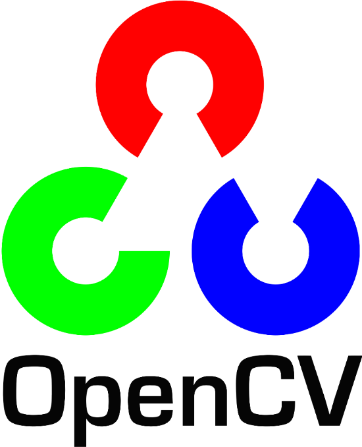
\includegraphics[width=0.5\linewidth]{images/image8.png}
    \end{center}
\end{figure}

\subsection{Scikit-learn}
[da https://en.wikipedia.org/wiki/Scikit-learn]
Scikit-learn (precedentemente conosciuto come scikits.learn e anche noto come sklearn) è una libreria di machine learning gratuita per il linguaggio di programmazione Python. 

Essa include vari algoritmi di classificazione, regressione e clustering, tra cui support-vector machine, random forest, gradient boosting, k-means e DBSCAN, ed è progettata per funzionare in combinazione con le librerie numeriche e scientifiche di Python, come NumPy e SciPy. 

Il progetto scikit-learn è nato come progetto Google Summer of Code dal data scientist francese David Cournapeau, originariamente chiamato scikits.learn. Il nome del progetto deriva dal concetto di "SciKit" (SciPy Toolkit), un'estensione di terze parti separata e distribuita per SciPy. 

Il codice originale è stato successivamente riscritto da altri sviluppatori. Nel 2010, i contribuenti Fabian Pedregosa, Gaël Varoquaux, Alexandre Gramfort e Vincent Michel dall'Istituto francese per la ricerca in informatica e automazione a Saclay, hanno preso il comando del progetto rilasciando in  seguito la prima versione pubblica della libreria il 1 febbraio 2010. Nel novembre 2012, scikit-learn e scikit-image sono stati descritti come due delle "scikits library" meglio conservate e popolari. 
Nel 2019 si è poi stimato che scikit-learn fosse una delle librerie di machine learning più popolari su GitHub.

Scikit-learn è principalmente scritto in Python e utilizza ampiamente NumPy per l'algebra lineare ad alta prestazione e le operazioni sugli array. 

Inoltre, alcuni algoritmi core sono scritti in Cython per migliorare le prestazioni. Support vector machine è implementato da un wrapper Cython intorno a LIBSVM; la regressione logistica e le macchine a vettori di supporto lineari da un wrapper simile intorno a LIBLINEAR. In tali casi, estendere questi metodi con Python potrebbe non essere possibile.

Scikit-learn si integra bene con molte altre librerie di Python come Matplotlib e Plotly per la visualizzazione dei dati, NumPy per la vettorizzazione degli array, Pandas dataframes, SciPy e molte altre.

\begin{figure}
    \begin{center}    
        
\includegraphics[width=0.7 \linewidth]{images/image9.png}
    \end{center}
\end{figure}

